%!TEX root = report.tex

\chapter{Experiments}
In this chapter we detail the experiments performed on the model described in
\fullref{chp:theorystuff} and discuss the respective results.

\section{??first experiment??}

% documentazione wrapfig: https://ctan.mirror.garr.it/mirrors/ctan/macros/latex/contrib/wrapfig/wrapfig-doc.pdf
% lo segno perché il primo parametro opzionale può tornare utile
\begin{wrapfigure}[17]{r}{0.5\textwidth}
    \centering
    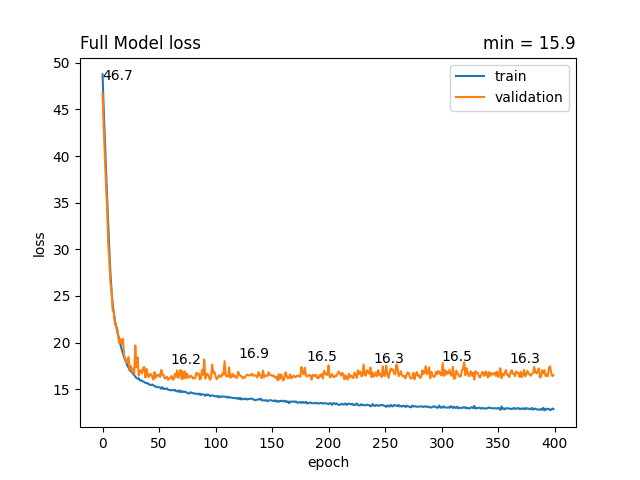
\includegraphics[width=0.5\textwidth]{400_loss}
    \caption{Initial experiment loss (400 epochs on Wiki)}
    \label{fig:400_loss}
\end{wrapfigure}

An initial experiment was performed by training the C3AE model for
400 epochs on the Wiki dataset as a means to test the \texttt{tensorflow} environment
and the functioning of the implemented C3AE model within it.

The evolution of training and validation loss is shown in \autoref{fig:400_loss}.
The experiment ran to completition with no runtime errors, and
it can be observed that the model was able to decrease its loss,
and that such loss reached an asymptote around epoch 50.

For this reason, we concluded that a training time of 400 epochs
is too much for this model and decided to set the epoch limit to 100 for
all following experiments, assuming that they would have a similar
evolution to this one and therefore all significant improvement
would happen much before the 100\textsuperscript{th} epoch,
in order to reduce the experiments' computation time.

\section{??other full experiments??}
????????????????????????

(One on Wiki, one on UTK, one on Wiki+UTK, all tested w/ FGNET)

????????????????????????

\section{Ablation Study}
A separate set of experiments was performed to study the impact on performance
of the following components of the model and the training process:
the context module and the cascade module of the C3AE model,
and the training data augmentation.

We trained the following variants of the full C3AE model:

\begin{itemize}
  \item \textit{Full model}: the standard model with no changes,
    to serve as a benchmark against the other variants.
  \item \textit{No augmentation}: the data augmentation transformations
    on the training data are disabled.
  \item \textit{No context}: the context module of C3AE is excluded.
    Therefore, only one crop, the outermost one, is given as input to
    the model, and obviously there is no concatenation phase.
  \item \textit{No cascade}: the cascade module of C3AE is excluded.
    Consequently, the intermediate layer between the concatenated feature vector
    and the age output loses its meaning of two-point representation of age
    and becomes a plain hidden layer. This also means that this variant
    does not compute any KL Divergence and outputs only the final age estimation;
    the loss depends only on the age MAE as well.
  \item \textit{No context and no cascade}: both modules are disabled.
\end{itemize}

Each variant was trained for 100 epochs on the Wiki dataset.
((Use of test set needs some debugging))

((plot and discuss results))
